\pagebreak

\section{Introduction}
\label{sec:introduction}

% state the learning objective
\paragraph{} 
The objective of this laboratory assignment is to study and implement an AC/DC converter circuit while, at the same time, trying to maximize the figure of merit M. The AC/DC converter circuit can be separated into two circuits: an Envelope Detector circuit, that takes a (relatively) high-frequency amplitude modulated signal as input and provides an output (the demodulated envelope of the original signal), and a Voltage Regulator circuit, designed to automatically maintain a constant voltage. The circuit can be seen in Figure~\ref{fig:circuit}.


The implementation of the AC-DC converter circuit was made according to the theoretical or simulation principles we were based on, with the construction of two simillar circuits with just a few differences in the components value (such as the resistance of some resistors and the capacitance of the capacitors) and also in the components number (such as the number of diodes). These small adjustments were made in order to compensate the changes in the behaviour of the electric circuits components verified while implementing both the theoretical circuit in GNU Octave and the simulation circuit in NGSpice.



\paragraph{}
In Section~\ref{sec:theoretical}, a theoretical introduction is made in order to contextualize all the main principles that sustain our construction and analysis of the circuit. A theoretical AC-DC coverter is built and carefully analysed in Section~\ref{sec:analysis}, where the results are obtained in GNU Octave. Also, in Section~\ref{sec:simulation}, another AC-DC converter is constructed and analysed by simulation through the use of NGSpice to simulate the real electric circuit behaviour. The results of the simulation of Section~\ref{sec:simulation} are then compared to the theoretical results obtained in Section~\ref{sec:analysis} and the comparative results are expressed in Section~\ref{sec:erroranalysis}. The figure of merit, calculated according to the components used to build the simulation circuit, can also be found in Section~\ref{sec:erroranalysis}. The conclusions of this study are outlined in the final part of the report, in Section~\ref{sec:conclusion}.


\begin{figure}[h] \centering
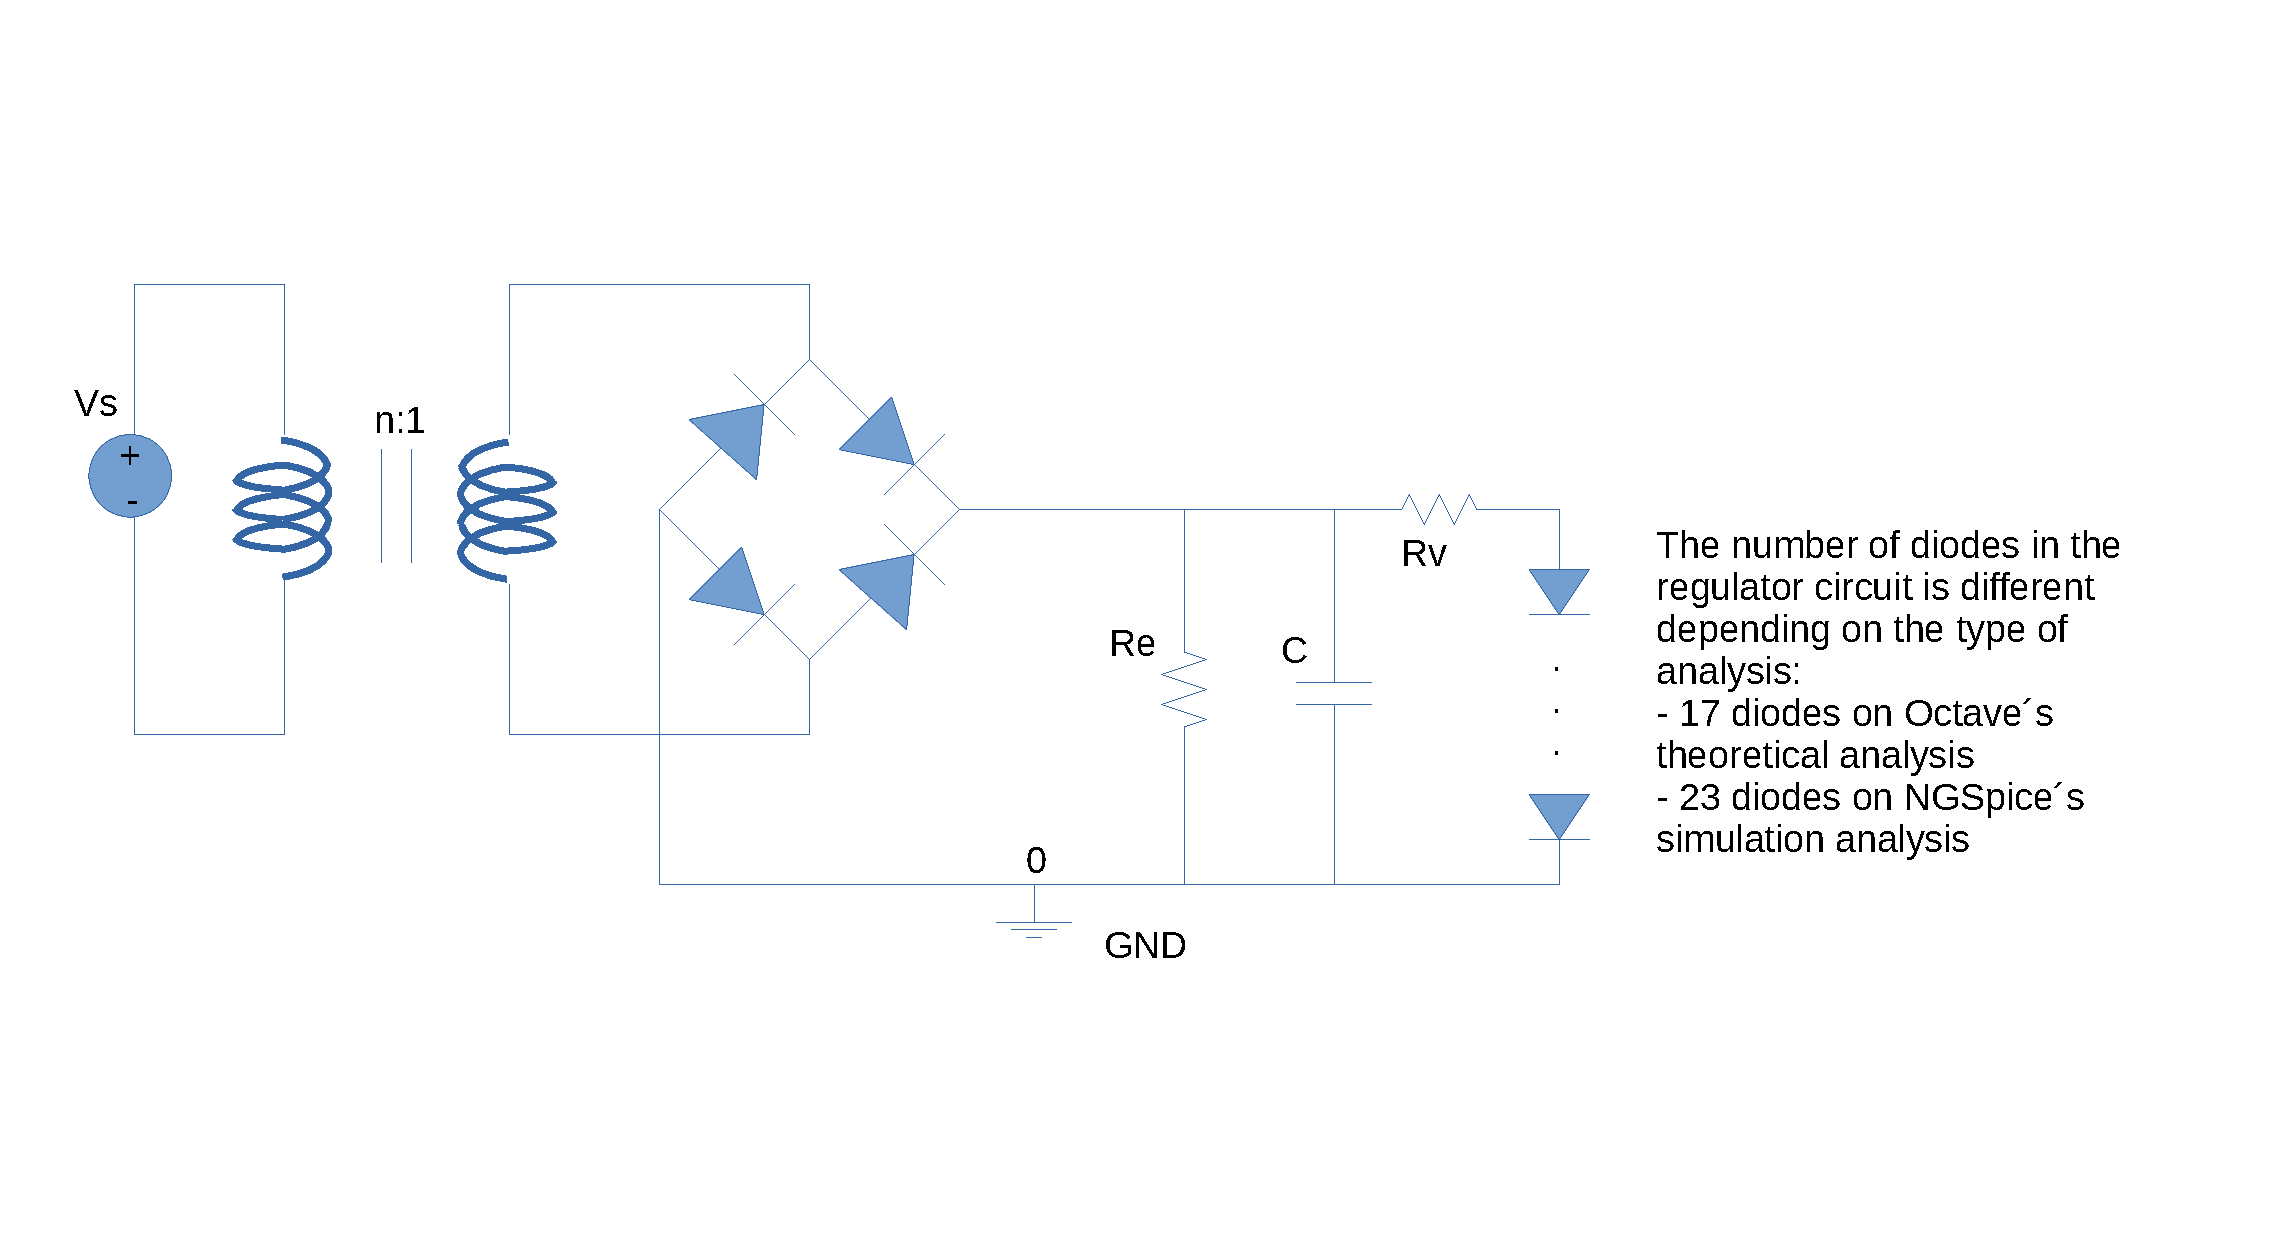
\includegraphics[width=0.8\linewidth]{circuit.pdf}
\caption{Third laboratory circuit.}
\label{fig:circuit}
\end{figure}

